\documentclass[11pt]{article}

\usepackage[margin=1in]{geometry}
\usepackage{graphicx}
\usepackage{caption}
\usepackage{hyperref}
\usepackage{booktabs}

\captionsetup{font=large, labelfont=bf}

\hypersetup{
  colorlinks=true,
  linkcolor=blue,
  urlcolor=blue,
  citecolor=blue
}

\title{Weekly Report: Photon Integration for Wafer-Scale GPU Simulation}
\author{Daoxuan Xu}
\date{May 11, 2026}

\begin{document}
\maketitle

\section{Summary}

\begin{itemize}
  \item Integrated Photon into the wafer-scale GPU simulation model.
  \item Verified that Photon works on the 3$\times$3 wafer-scale GPU model.
  \item Evaluated Photon on the 7$\times$7 wafer-scale GPU model.
  \item Collected a broader 7$\times$7 sampled-validation run across multiple
        benchmarks.
  \item Found that matrix multiplication and matrix transpose have too few
        workgroups for effective sampling on 7$\times$7.
  \item Tried modified matrix benchmarks with more workgroups, but the first
        small-tile version reduced CU utilization.
  \item Started a loop-level sampling prototype.
\end{itemize}

\section{Main Results}

Photon is a sampled-simulation mechanism. It first runs part of the workload in
detailed mode, checks whether the execution time has become stable, and then
uses the measured timing to predict later repetitive work instead of simulating
every wavefront in detail.

Photon has three sampling levels:

\begin{itemize}
  \item \textbf{Wavefront-level sampling} (\texttt{sample\_wf},
        \texttt{-sampled}): Photon observes detailed wavefront issue and finish
        times. Once the timing window becomes stable, it predicts later
        wavefronts using the sampled average time. This level is effective when
        a kernel launches many similar wavefronts.
  \item \textbf{Branch-level sampling} (\texttt{sample\_branch},
        \texttt{-branch-sampled}): Photon tracks basic-block and branch
        behavior inside wavefronts. When the basic-block coverage is high enough
        and the timing model is stable, it predicts repeated instruction
        regions instead of simulating every instruction path in detail.
  \item \textbf{Kernel-level sampling} (\texttt{sample\_kernel},
        \texttt{-kernel-sampled}): Photon compares the current kernel behavior
        with previous kernel history. If the wavefront/BBV pattern is close
        enough to a known history, it predicts a larger part of the kernel. This
        is the coarsest level and can provide high speedup when kernels are
        repetitive.
\end{itemize}

\texttt{sample\_all} enables all three levels together. In this report, the key
parameters are:

\begin{itemize}
  \item \textbf{Warmup}: the number of detailed wavefronts collected before
        Photon starts fitting the sampled timing model.
  \item \textbf{Granularity}: the size of the stability window used to decide
        whether the sampled timing is stable enough for prediction.
\end{itemize}

For example, \texttt{w128\_g256} means \texttt{sampled-warmup=128} and
\texttt{sampled-granularity=256}. Larger values are more conservative and can
reduce the error rate, while smaller values can enable earlier skipping and
improve simulator speedup.

\subsection{Photon Validation}
To validate that Photon works in the wafer-scale GPU model, I first tested it
on the 3$\times$3 configuration. Figure~\ref{fig:relu-3x3} shows the ReLU
sampling sweep. Some configurations achieve about 2--2.6$\times$ wall-clock
speedup while keeping the simulation error rate below 5\%.
The result also shows that the warmup and granularity hyperparameters are
important during sampling.

\begin{figure}[h]
  \centering
  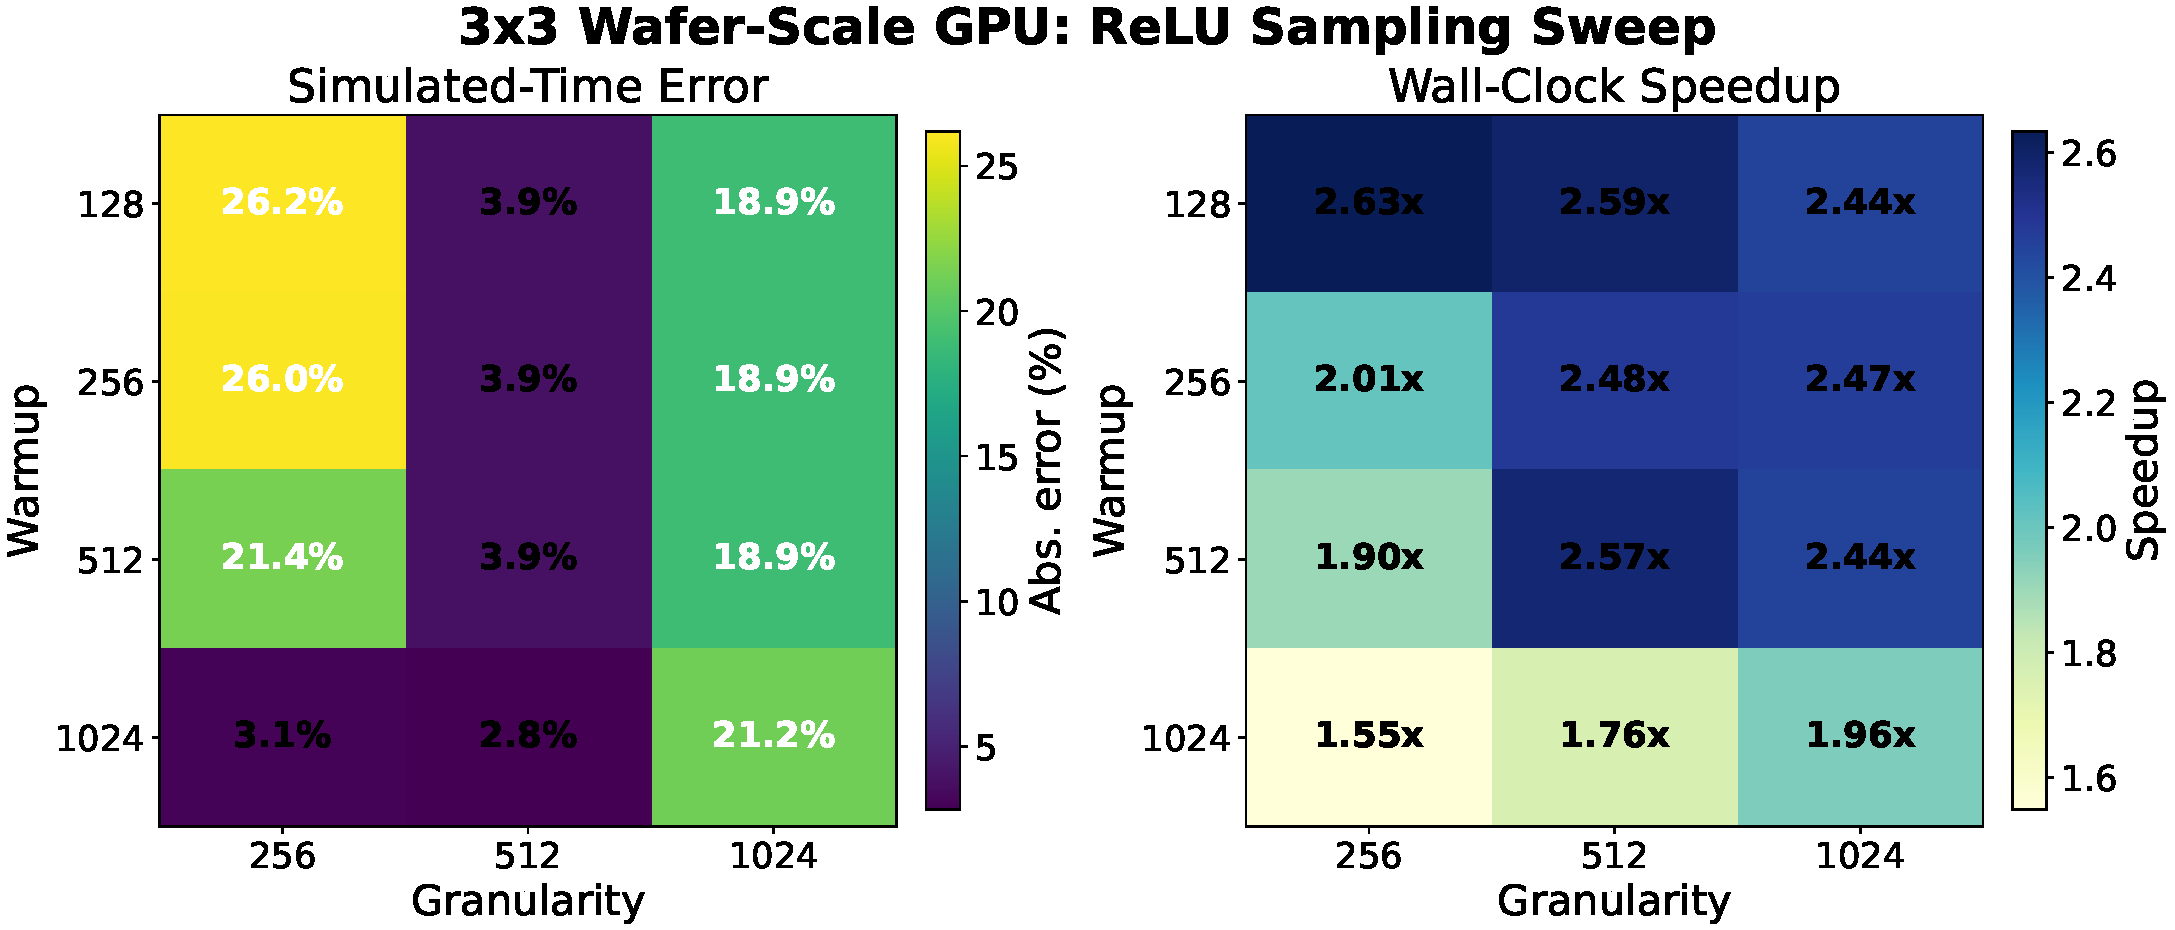
\includegraphics[width=\linewidth]{figures/relu_3x3_tradeoff_large.pdf}
  \caption{ReLU sampled-simulation tradeoff on the 3$\times$3 wafer-scale GPU model.}
  \label{fig:relu-3x3}
\end{figure}

\subsection{Experiment on 7$\times$7 size model}
Table~\ref{tab:wg-7x7} summarizes the workgroup count for each benchmark in the
7$\times$7 run. This table helps explain why Photon does not work well for
matrix multiplication. Matrix multiplication has only 65,536 total WGs, or 43 WGs/CU,
which is much lower than workloads such as ReLU and im2col. After
Photon spends time on warmup and stability detection, there are too few
remaining workgroups to skip, so the simulator speedup is limited.

\begin{table}[h]
  \centering
  \small
  \begin{tabular}{lrr}
    \toprule
    Benchmark & Total WG & WG/CU \\
    \midrule
    % pagerank & 3,276,800 & 2,134 \\
    im2col & 2,093,060 & 1,363 \\
    simpleconvolution & 1,049,665 & 684 \\
    floydwarshall & 1,048,576 & 683 \\
    relu & 983,040 & 640 \\
    % bitonicsort & 524,288 & 342 \\
    aes & 409,600 & 267 \\
    fir & 272,000 & 178 \\
    % fastwalshtransform & 131,072 & 86 \\
    fft & 98,304 & 64 \\
    matrixmultiplication & 65,536 & 43 \\
    % spmv & 65,536 & 43 \\
    % kmeans & 51,200 & 34 \\
    % \textbf{matrixtranspose} & \textbf{16,384} & \textbf{11} \\
    \bottomrule
  \end{tabular}
  \caption{Workgroup count of each benchmark .}
  \label{tab:wg-7x7}
\end{table}

Figure~\ref{fig:success-7x7} shows the broader 7$\times$7 validation run with
benchmarks that completed successfully. Photon gives clear simulator speedup
for several workloads, but some workloads still have high error rates. For
example, ReLU and im2col are faster, but their error rates are above 10\%.

\begin{figure}[h]
  \centering
  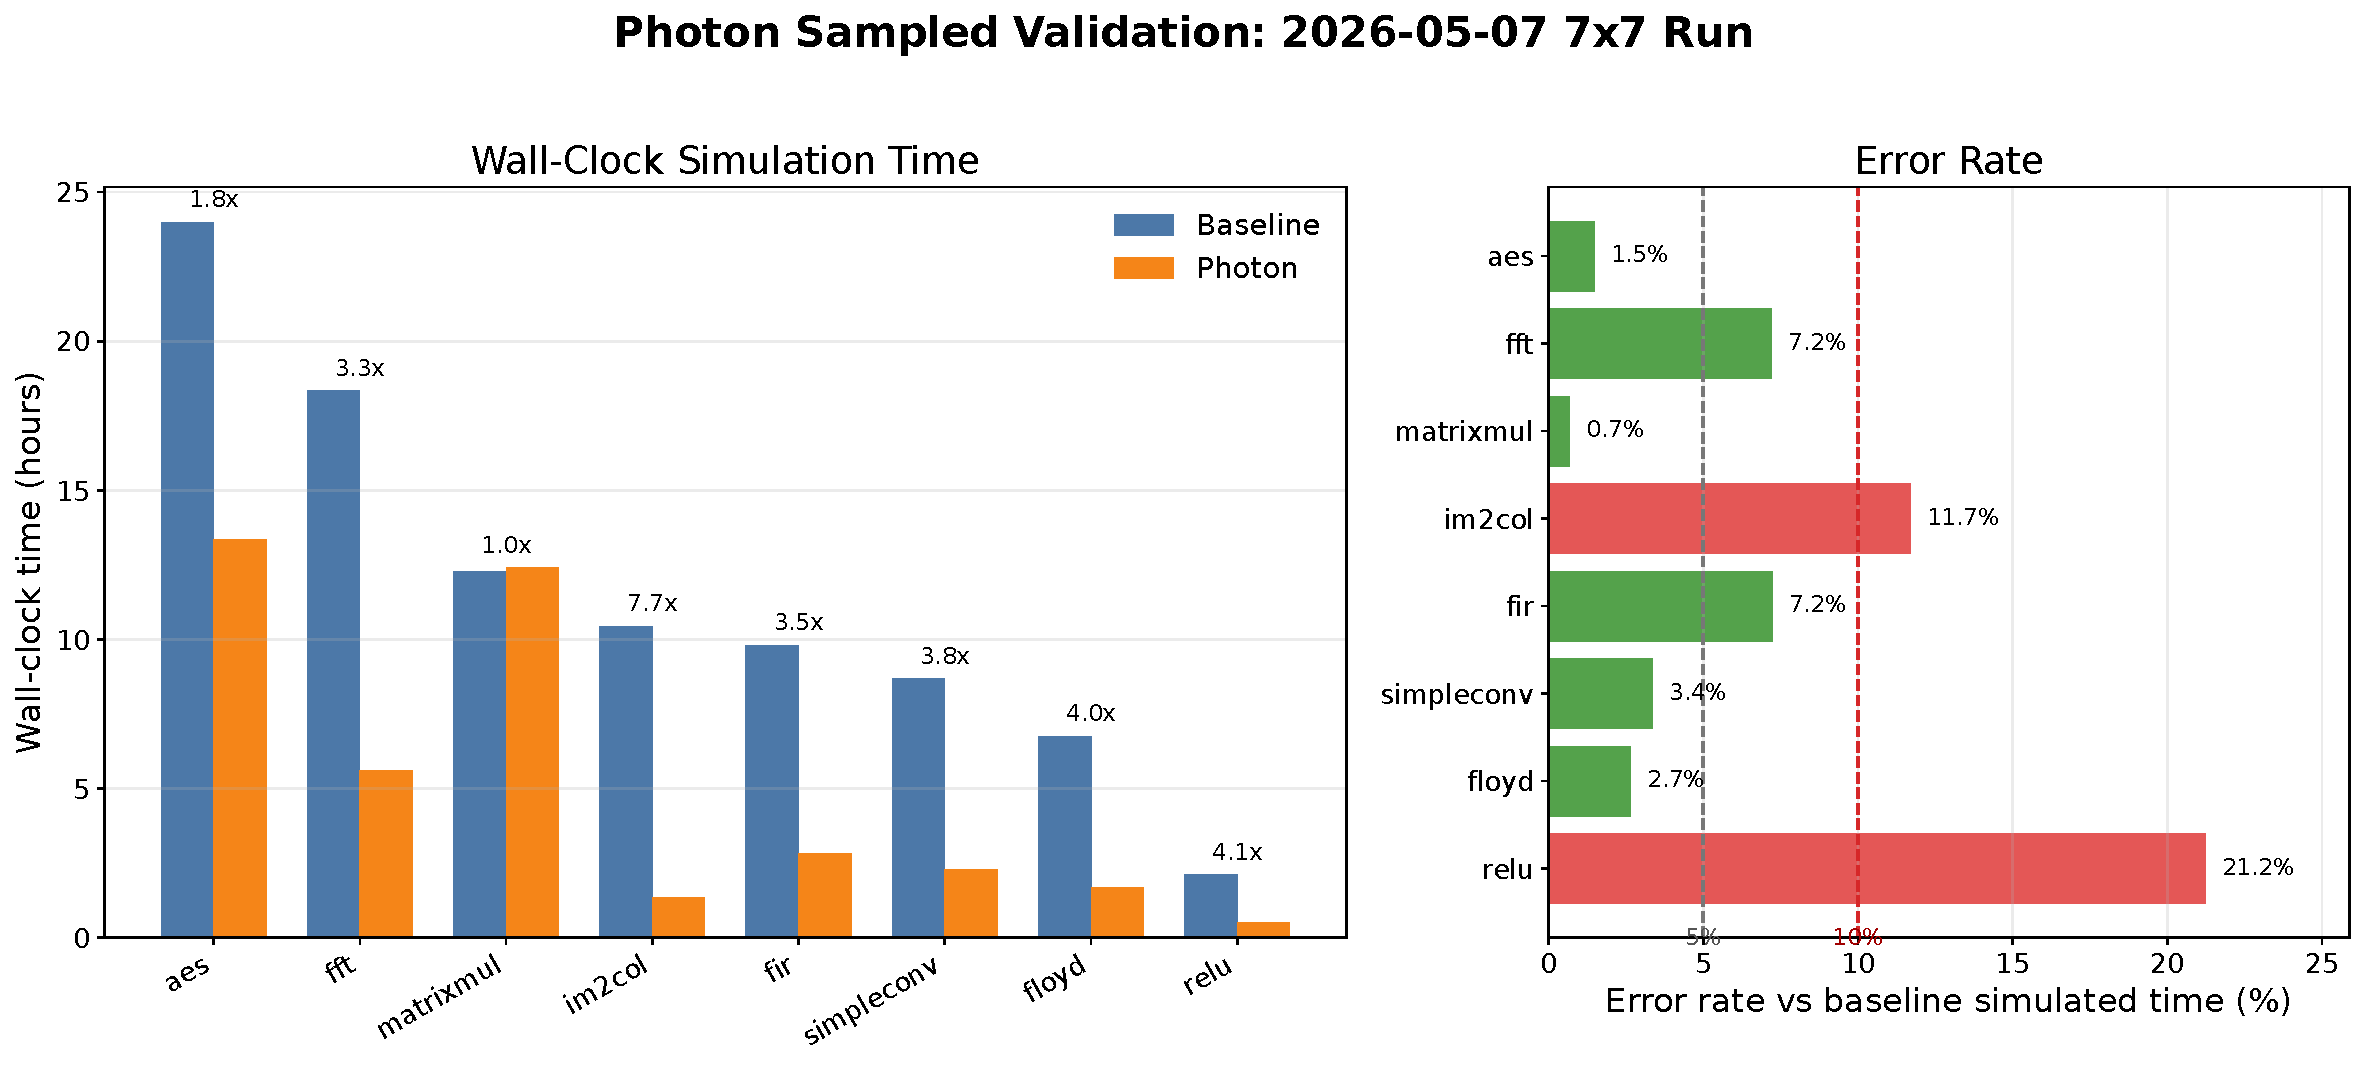
\includegraphics[width=\linewidth]{figures/photon_2026_05_07_success_large.pdf}
  \caption{Wall-clock speedup and simulated-time error rate for successfully
  completed workloads in the 2026-05-07 7$\times$7 run. (warmup 128 wg, granularity 4096wg).}
  \label{fig:success-7x7}
\end{figure}

\subsection{Benchmark Modification}
As shown in Figure~\ref{fig:workload-7x7}, ReLU gets a large speedup because it
has much more per-CU work. Matrix multiplication and matrix transpose get
smaller speedups because after sampling finishes, there are not enough
remaining workgroups to skip. Although the exact WG count can change across
benchmark versions, the main limitation is the same: the matrix workloads have
too little remaining work per CU to amortize Photon warmup and prediction
overhead.

\begin{figure}[h]
  \centering
  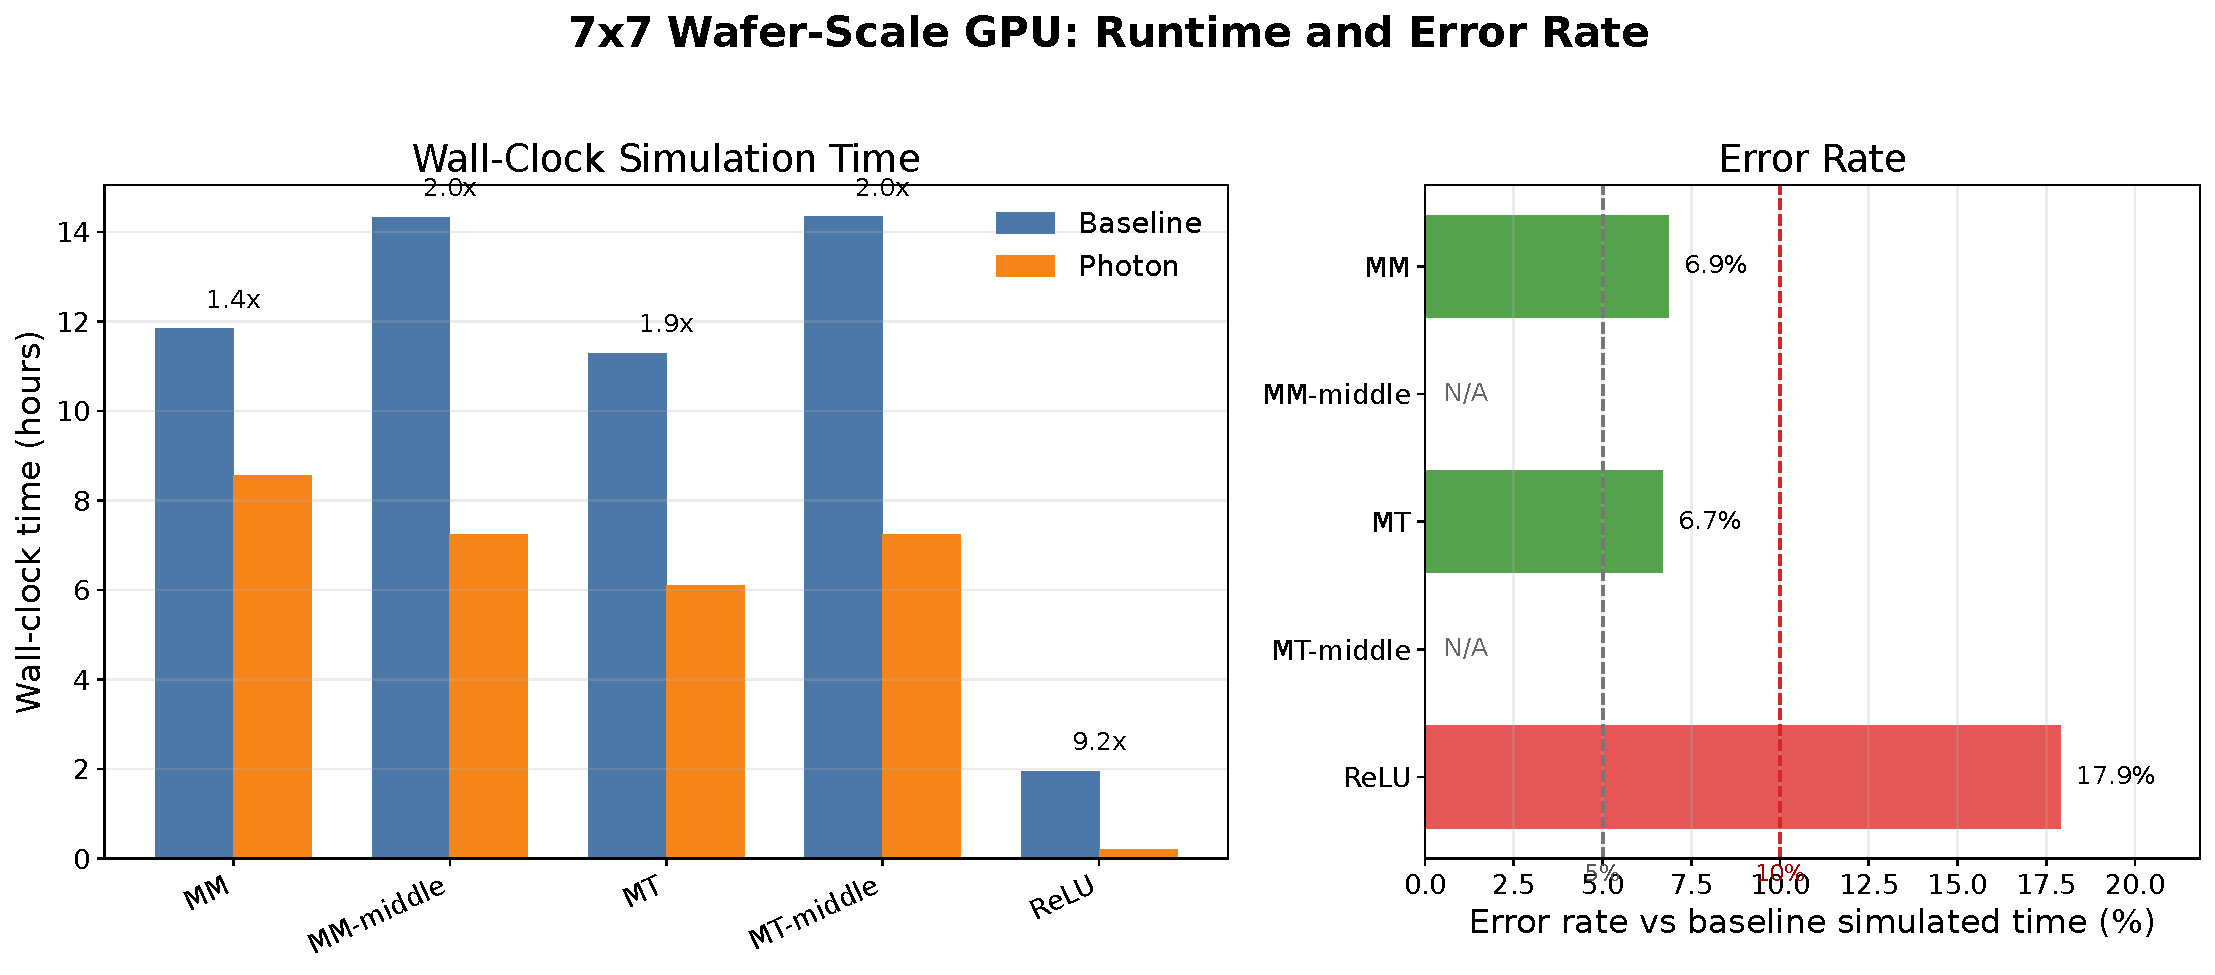
\includegraphics[width=\linewidth]{figures/workload_time_error_large.pdf}
  \caption{Wall-clock simulation time and simulated total-time error rate on the
  7$\times$7 wafer-scale GPU model. The error rate is measured against baseline
  \texttt{Driver,total\_time}.}
  \label{fig:workload-7x7}
\end{figure}

% \section{Benchmark Modification}

I modified the matrix benchmarks to generate more workgroups without increasing
the problem size or memory footprint. The main idea is to reduce the amount of
output computed by each workgroup, so the same matrix problem is decomposed into
more workgroups.

\begin{table}[h]
  \centering
  \small
  \begin{tabular}{lcccc}
    \toprule
    Benchmark & Original tile & Small tile & Middle tile & Effect \\
    \midrule
    Matrix multiplication & 8$\times$8 & 4$\times$4 & 8$\times$4 &
      4$\times$ / 2$\times$ more WGs \\
    Matrix transpose & 16$\times$16 & 4$\times$4 & 8$\times$8 &
      16$\times$ / 4$\times$ more WGs \\
    \bottomrule
  \end{tabular}
  \caption{Small-tile and middle-tile matrix workload modifications for
  increasing workgroup count while keeping the same problem size. The effect
  column reports small-tile / middle-tile workgroup-count increase.}
  \label{tab:matrix-modification}
\end{table}

The first attempt was an aggressive small-tile version. For matrix
multiplication, I changed the workgroup from 8$\times$8 to 4$\times$4. This
increased the workgroup count from 65,536 to 262,144, or from 43 to 171 WGs/CU.
For matrix transpose, I changed the workgroup from 16$\times$16 to 4$\times$4.
This increased the workgroup count from 65,536 to 1,048,576, or from 43 to 683
WGs/CU. However, each small-tile workgroup has only 16 work-items, so it cannot
fill a 64-lane wavefront. This reduced CU utilization and made the benchmark
slower.

The middle-tile version is a compromise. In the 2026-05-11 run, this
modification increased matrix multiplication from 65,536 to 131,072 WGs, or
from 43 to 86 WGs/CU. For matrix transpose, it increased the count from 65,536
to 262,144 WGs, or from 43 to 171 WGs/CU.

For matrix multiplication, the vanilla kernel uses an 8$\times$8 workgroup. The
middle-tile version keeps the same matrix dimensions
(\texttt{X=256, Y=2048*128, Z=256}) but changes the workgroup shape to
8$\times$4. Since the global work size is unchanged, halving the local
workgroup height roughly doubles the number of workgroups.

For matrix transpose, the vanilla kernel uses a 16$\times$16 workgroup with four
elements per thread in each dimension. The middle-tile version keeps the same
matrix width (\texttt{Width=8192*2}) but changes the block size from 16 to 8.
This changes the workgroup from 16$\times$16 to 8$\times$8. Since both tile
dimensions are halved, the total number of workgroups increases by about
4$\times$.

This creates more workgroups for Photon to sample and skip, but it also reduces
the amount of work in each workgroup. Therefore, there is a tradeoff between
having enough workgroups for sampling and keeping enough per-workgroup work to
utilize the CUs. The first aggressive small-tile version reduced CU utilization.
For matrix transpose:

\begin{itemize}
  \item Vanilla matrix transpose: \texttt{0.028275329000}
  \item Modified small-tile matrix transpose: \texttt{0.118611286000}
\end{itemize}

The modified version is about 4.2$\times$ slower. This suggests that simply
increasing the number of workgroups is not enough; each workgroup also needs
enough work to keep the CUs busy.

\section{Loop-Level Sampling}

I started implementing loop-level sampling as a possible solution. The current
prototype detects backward branches and checks whether loop iteration time
becomes stable. The next step is to test whether stable loops can be skipped
correctly.

\section{Next Steps}

\begin{itemize}
  \item Test whether loop-level sampling works and measure its error rate and speedup.
  \item Build LLM workloads such as BERT, GPT-2, T5, and LLaMA.
\end{itemize}

\end{document}
